
\section*{Other Frameworks: Trike, VAST, OCTAVE, and OWASP}
Threat modeling is a diverse and evolving discipline, with several frameworks developed to address different organizational, technical, and regulatory needs. This chapter explores four important alternatives to STRIDE and PASTA, providing technical definitions, strengths, limitations, and practical application guidance\cite{owasp,nist800154}.

\subsection*{Trike}
Trike is a risk management and threat modeling framework that focuses on defining acceptable risk and generating threat models based on system requirements. It uses three core models:\cite{uceda2015}
\begin{itemize}
	\item \textbf{Requirement Model:} Defines what is allowed and expected in the system.
	\item \textbf{Attack Model:} Identifies what can go wrong, mapping attacker actions to system components.
	\item \textbf{Risk Model:} Quantifies the impact and likelihood of threats, supporting risk-based decision making.
\end{itemize}
	extbf{Strengths:} Quantitative risk analysis, strong requirements focus.\\
	extbf{Limitations:} Less intuitive for developers, limited tool support.

\subsection*{VAST (Visual, Agile, and Simple Threat)}
VAST is designed for scalability and integration with agile/DevOps workflows. It uses visual diagrams to model both application and operational threats, making it suitable for large organizations with complex systems. VAST emphasizes automation and continuous threat modeling.\cite{owasp}
	extbf{Strengths:} Scalable, visual, integrates with CI/CD.\\
	extbf{Limitations:} Less detailed adversary simulation than PASTA.

\subsection*{OCTAVE (Operationally Critical Threat, Asset, and Vulnerability Evaluation)}
OCTAVE, developed by Carnegie Mellon, focuses on organizational risk and asset-based analysis. It aligns security with business objectives and is often applied at the enterprise level.\cite{nist800154}
	extbf{Strengths:} Business alignment, asset focus, strategic.\\
	extbf{Limitations:} Less technical detail, not ideal for application-level threats.

\subsection*{OWASP Threat Modeling}
OWASP provides a wealth of resources, including the Threat Modeling Cheat Sheet, which offers practical guidance, checklists, and templates. OWASP’s approach is community-driven and emphasizes actionable steps for developers and security teams.\cite{owasp}
	extbf{Strengths:} Practical, widely adopted, open-source resources.\\
	extbf{Limitations:} Not a formal framework, but a collection of best practices.

\subsection*{Framework Comparison Table}
\begin{table}[H]
\centering
\begin{tabular}{|l|l|l|l|}
\hline
	extbf{Framework} & \textbf{Focus} & \textbf{Best For} & \textbf{Limitation} \\
\hline
STRIDE & App threats & Dev/design teams & Less business focus \\
PASTA & Risk/attacker & Regulated, high-value & Resource intensive \\
Trike & Risk quantification & Auditors, risk managers & Steep learning curve \\
VAST & Scalability & Large, agile orgs & Less adversary detail \\
OCTAVE & Org risk & Enterprise, strategy & Not app-level \\
OWASP & Practical steps & Devs, SMEs & Not a full framework \\
\hline
\end{tabular}
\caption{Comparison of Threat Modeling Frameworks\cite{owasp,uceda2015,nist800154}}
\end{table}

\begin{figure}[H]
	\centering
	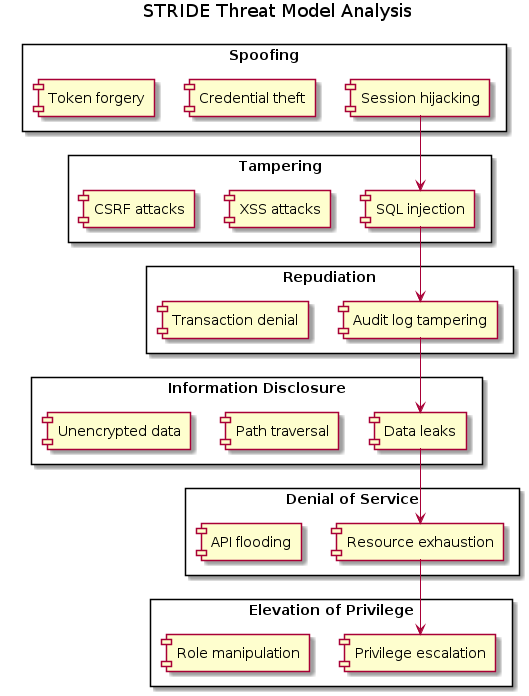
\includegraphics[width=0.8\textwidth]{images/stride-analysis}
	\caption{Visual Comparison of Threat Modeling Frameworks}
\end{figure}
